\documentclass{standalone}
\usepackage{tikz}
\begin{document}

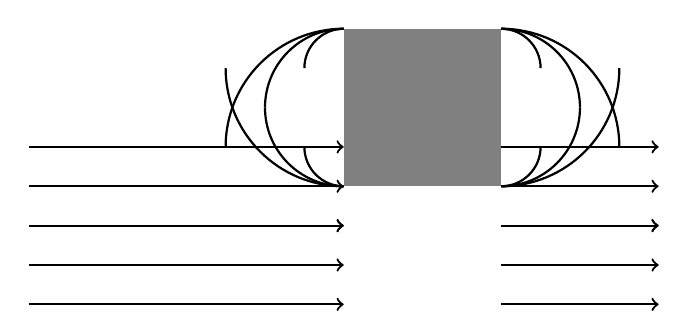
\begin{tikzpicture}
    % Zeichne das Quadrat (Hindernis)
    \fill[gray] (2, 2) rectangle (4, 4);
    
    % Wellenfronten vor dem Hindernis
    \foreach \x in {0.5, 1, 1.5} {
        \draw[thick, ->] (-2, \x) -- (2, \x);
        \draw[thick, ->] (-2, \x+1) -- (2, \x+1);
    }

    % Wellenfronten hinter dem Quadrat, gebeugte Wellen
    \foreach \r in {0.5, 1, 1.5} {
        % oben links
        \draw[thick] (2, 4) arc[start angle=90, end angle=180, radius=\r];
        % unten links
        \draw[thick] (2, 2) arc[start angle=-90, end angle=-180, radius=\r];
        % oben rechts
        \draw[thick] (4, 4) arc[start angle=90, end angle=0, radius=\r];
        % unten rechts
        \draw[thick] (4, 2) arc[start angle=-90, end angle=0, radius=\r];
    }

    % Erweiterte Wellenfronten nach dem Hindernis
    \foreach \x in {0.5, 1, 1.5} {
        \draw[thick, ->] (4, \x) -- (6, \x);
        \draw[thick, ->] (4, \x+1) -- (6, \x+1);
    }
\end{tikzpicture}

\end{document}